\documentclass[journal]{IEEEtran}

\usepackage{amsmath,amssymb}
\usepackage{array}
\usepackage{booktabs}
\usepackage{cite}
\usepackage{graphicx}
\usepackage{tabularx}
\usepackage{url}

\graphicspath{{figures/}}
\newcolumntype{Y}{>{\raggedright\arraybackslash}X}
\newcommand{\method}[1]{\texttt{\detokenize{#1}}}
\newcommand{\compactmethod}[1]{{\footnotesize\method{#1}}}
\newcommand{\primarymethod}{{\footnotesize\texttt{ts\_\allowbreak entropy\_\allowbreak cosine\_\allowbreak euclidean}}}
\newcommand{\exploratorymethod}{{\footnotesize\texttt{ts\_\allowbreak entropy\_\allowbreak cosine\_\allowbreak euclidean\_\allowbreak mahalanobis}}}
\newcommand{\pendingcite}[1]{\cite{#1}\,\textbf{[REFERENCE NEEDED: #1]}}
\newcommand{\submissionplaceholder}[1]{\textit{[Placeholder: #1]}}
\hyphenation{OpenEW-SA ElectroSense DeepSense JamShield}

\title{Uncertainty-Calibrated Multi-View RF Signal Recognition for Open-Set Electromagnetic Spectrum Monitoring}

\author{%
  \textbf{[AUTHOR PLACEHOLDER(S)]}%
  \thanks{\textbf{[AFFILIATION PLACEHOLDER(S)]}}%
  \thanks{Corresponding author: \textbf{[CORRESPONDING AUTHOR AND EMAIL PLACEHOLDER]}.}%
  \thanks{ORCID: \textbf{[AUTHOR ORCID PLACEHOLDER(S)]}.}%
  \thanks{Funding: \textbf{[FUNDING AGENCY, PROGRAM, AND GRANT NUMBER PLACEHOLDER]}.}%
}

\begin{document}

\maketitle

\begin{abstract}
Electromagnetic spectrum monitors encounter signal classes, receivers, acquisition days, and interference scenarios that are absent from closed-set training data. A recognizer can therefore be accurate and apparently well calibrated on retained in-distribution (ID) samples while assigning unwarranted confidence to operationally novel observations. This study develops a reproducible open-set evaluation path over existing OpenEW-SA processed artifacts from ElectroSense, DeepSense, and JamShield. The approach combines a calibrated predictive-uncertainty view with train-fitted feature-geometry views. A scalar temperature is fitted only on ID validation predictions; temperature-scaled entropy, nearest-centroid cosine distance, and nearest-centroid Euclidean distance are then normalized using validation-only robust statistics and averaged to form the prespecified primary score, \primarymethod. A variant that additionally includes Mahalanobis distance is retained as an exploratory ablation. All scores use a fixed higher-is-more-OOD orientation, and evaluation OOD labels are not used to choose orientations, weights, methods, or thresholds. Stratified paired bootstrap analysis shows that the primary fusion is effective for ElectroSense class novelty and improves AUROC against the prespecified comparators for JamShield scenario shift. JamShield nevertheless exhibits an operating-metric trade-off: AUPR-OOD and FPR95 are not uniformly better against every comparator. DeepSense remains a negative fixed-orientation result, indicating that a held-out acquisition day can appear more geometrically typical than retained ID data. Post-hoc score negation is reported only as a diagnostic and does not replace the primary result. These findings support a dataset-dependent view of uncertainty-distance fusion and show that closed-set calibration alone does not ensure robust OOD separation.
\end{abstract}

\begin{IEEEkeywords}
RF signal recognition, electromagnetic spectrum monitoring, out-of-distribution detection, open-set recognition, uncertainty calibration, temperature scaling, feature distance, score fusion.
\end{IEEEkeywords}

\section{Introduction}
\label{sec:introduction}

Electromagnetic spectrum monitoring systems are expected to recognize known activity while operating across changing emitters, receivers, sites, propagation conditions, acquisition schedules, and interference regimes. Conventional supervised recognition assumes that evaluation samples belong to the same label and domain support as the training set. That assumption is fragile in open-spectrum operation, where an unknown signal technology, a new acquisition domain, or a previously unseen jammer scenario may be encountered without an OOD label available at decision time. Closed-set models can remain confident under such shifts, so classification confidence and OOD separability must be evaluated as related but distinct properties. \pendingcite{R1} \pendingcite{R2}

RF OOD evaluation also has a protocol-design problem. An apparent detector can be improved after the fact by reversing a score, selecting the strongest test comparator, fitting normalization on evaluation samples, or optimizing a threshold using OOD labels. Those operations leak information from the target shift and can turn a diagnostic observation into an overstated primary result. A deployment-relevant experiment instead fixes the score direction and analysis roles in advance, fits classifiers and distance models on training data, fits calibration and normalization on ID validation data, and leaves the test ID and test OOD rows untouched until evaluation. \pendingcite{R3}

This work studies that disciplined path on the OpenEW-SA artifact convention. The term \emph{multi-view} has two scopes here. Across datasets, the evaluation includes processed power-spectral-density (PSD), in-phase/quadrature (I/Q), and tabular radio/network representations. Within the proposed detector, the fused views are complementary evidence sources: predictive uncertainty and two forms of feature-space distance. The current experiments do not claim an end-to-end, within-sample fusion of raw I/Q, PSD, spectrogram, and metadata inputs; that broader multimodal model remains future work.

The study makes four contributions. First, it defines frozen class-OOD and domain/scenario-OOD evaluations for ElectroSense, DeepSense, and JamShield while preserving symbolic RF labels. Second, it connects a lightweight supervised recognition baseline, validation-fitted temperature scaling, and train-fitted feature-distance scores in one reproducible pipeline. Third, it specifies \method{ts_entropy_cosine_euclidean} as an equal-weight primary fusion after ID-validation-only robust normalization, while keeping the Mahalanobis-augmented fusion exploratory. Fourth, it reports fixed-orientation point estimates and paired bootstrap uncertainty, including a negative DeepSense result and a post-hoc inversion diagnostic that is explicitly excluded from the primary analysis.

The resulting evidence is intentionally bounded. The primary method performs differently across the three shifts, and no universal generalization or universal statistical-significance claim is made. Instead, the analysis asks where calibrated uncertainty and feature geometry agree, where they trade off across metrics, and where their assumed higher-is-more-OOD direction breaks under domain change.

\section{Related Work}
\label{sec:related-work}

\subsection{Open-Set and OOD Recognition for RF Monitoring}

Open-set recognition distinguishes known-class classification from the additional requirement to reject observations outside the modeled class support. OOD detection broadens the concern to covariate and domain shifts that can preserve labels while changing the observation distribution. Both settings are relevant to RF monitoring because waveform, sensor, site, day, channel, and interference changes can alter the feature distribution independently of the nominal recognition task. A final version should cite foundational open-set/OOD work and RF-specific evaluations rather than treating computer-vision evidence as automatically transferable. \pendingcite{R4} \pendingcite{R5}

\subsection{Confidence and Calibration}

Maximum softmax probability, predictive entropy, and logit-energy scores are common post-hoc confidence baselines because they can be computed from an existing classifier without retraining an explicit OOD model. Temperature scaling fits a scalar on held-out ID predictions to improve probabilistic calibration while leaving the classifier architecture fixed. These techniques address different properties: calibration concerns the relationship between confidence and correctness on a specified distribution, whereas OOD detection concerns ranking or separating a shifted population. Their relationship should therefore be tested rather than assumed. \pendingcite{R6} \pendingcite{R7} \pendingcite{R8}

\subsection{Feature Geometry and Score Fusion}

Prototype and Mahalanobis approaches score a sample by its position relative to class-conditional training features. Euclidean and cosine distances encode different geometry, while a shared-covariance Mahalanobis score adjusts directions by estimated within-class variability. Their usefulness depends on whether novelty actually maps to increasing distance in the learned or processed representation. Combining uncertainty and distance can expose complementary evidence, but score scales must be aligned without consulting evaluation OOD labels. \pendingcite{R9} \pendingcite{R10}

\subsection{Statistical Evaluation of OOD Scores}

AUROC, AUPR with OOD as the positive class, and FPR at a high OOD true-positive rate summarize different aspects of ranking and operating behavior. Paired resampling is useful when competing methods score exactly the same observations because a shared resample preserves within-sample dependence. Confidence intervals nevertheless quantify uncertainty conditional on the observed dataset and resampling design; they do not establish performance on every future domain. \pendingcite{R11} \pendingcite{R12}

\section{Datasets and OOD Evaluation Protocols}
\label{sec:datasets}

The experiments use converted OpenEW-SA artifacts with one metadata row per sample, an index into a shared feature array, and symbolic labels loaded as strings. Each frozen protocol contains an ID training split, an ID validation split, an ID test split, and an OOD test split. The evaluation CSV is the concatenation of test ID and test OOD rows only. Table~\ref{tab:dataset-protocols} reports the verified evaluation counts used by every compared v3 method.

\begin{table*}[!t]
  \caption{Dataset and OOD protocol summary. Processed input view, recognition target, frozen OOD definition, and verified ID/OOD evaluation counts for ElectroSense, DeepSense, and JamShield. Counts refer to the frozen evaluation set, not the training or validation partitions.}
  \label{tab:dataset-protocols}
  \centering
  \scriptsize
  \setlength{\tabcolsep}{3pt}
  \renewcommand{\arraystretch}{1.12}
  \begin{tabularx}{\textwidth}{@{}l l l l Y Y r r r@{}}
    \toprule
    Dataset & Input & Target & Protocol & ID definition & OOD definition & ID & OOD & Total \\
    \midrule
    ElectroSense & PSD & Signal technology & Class OOD &
      DAB, DVB-T, FM, and LTE classes &
      GSM and TETRA classes &
      5,840 & 16,550 & 22,390 \\
    DeepSense & I/Q & Wi-Fi occupancy code & Acquisition-day OOD &
      Retained day-one samples &
      Held-out day-two samples &
      3,200 & 16,000 & 19,200 \\
    JamShield & Tabular radio/network metrics & Normal versus abnormal interference & Scenario OOD &
      Retained benign and jammer scenarios &
      Held-out benign and jammer scenarios &
      14,534 & 19,817 & 34,351 \\
    \bottomrule
  \end{tabularx}
\end{table*}


\subsection{ElectroSense Class OOD}

ElectroSense provides crowdsensed PSD data and an official wireless-technology classification framework~\cite{rajendran2018electrosense,scalingi2023framework,scalingi2023electrosensepsd}. The taxonomy and split used here are scoped to the converted OpenEW-SA subset: DAB, DVB-T, FM, and LTE are treated as known classes for classifier fitting and ID evaluation, while GSM and TETRA are withheld from classifier training and treated as OOD at evaluation. The upstream framework code also defines an \method{unkn} label; the analyzed frozen manifest and split artifacts contain only the six named technology labels and therefore exclude \method{unkn}. This six-class construction is not attributed to the Zenodo record itself.

\subsection{DeepSense Acquisition-Day OOD}

DeepSense contributes processed I/Q windows labeled by binary occupancy codes~\cite{uvaydov2021deepsense,wineslab2021deepsensedataset}. All occupancy codes remain known labels, while the acquisition day defines the shift: retained day-one rows provide train, validation, and test-ID samples, and held-out day-two rows provide OOD samples. Labels such as \method{0000}, \method{0001}, \method{0010}, and \method{0100} are identifiers and are read and written as strings so their leading zeros cannot be lost. This protocol tests domain shift rather than unseen-class rejection; the official dataset record documents different transmitter orientations across the two acquisition days.

\subsection{JamShield Scenario OOD}

JamShield contributes tabular radio and network telemetry for normal-versus-abnormal interference recognition~\cite{panitsas2025jamshield,panitsas2024jamshielddataset}. Both recognition labels occur in the retained scenarios, while a frozen subset of benign and jammer scenarios is held out as OOD. The task therefore asks whether a classifier and its training geometry can identify scenario novelty even when the nominal label vocabulary remains unchanged. The exact retained and held-out domain identifiers are fixed in the split manifests. The peer-reviewed ICC 2025 publication is cited for the system, while the public dataset record supports the scenario and telemetry provenance; no explicit dataset license was identified in the verified public records.

\subsection{Leakage Controls}

Training features and labels are used to fit the classifier and the class centroids. ID validation predictions are used to fit temperature scaling, and ID validation component scores are used to fit score normalization. Test-ID and test-OOD labels are used only for final metric computation, audit alignment, and the explicitly labeled post-hoc DeepSense diagnostic. They are not used to choose the score orientation, normalization statistics, fusion weights, primary method, comparator set, or a deployment threshold.

\section{Methods}
\label{sec:methods}

\subsection{Notation and Fixed Score Orientation}

Let \(x\) denote a processed RF feature vector, \(y\) a known-class label, \(p_k(x)\) the classifier probability for class \(k\), and \(z(x)\) the feature representation used by the classifier and distance models. Every OOD component is oriented before evaluation so that a larger value means more OOD-like. This convention is retained even when a dataset produces an inverted ranking. OOD labels do not enter any score definition.

\subsection{Baseline Confidence Scores}

The supervised baseline produces class probabilities and a predicted label for each validation and evaluation sample. The maximum-softmax-probability OOD score is implemented as
\begin{equation}
  s_{\mathrm{MSP}}(x) = 1 - \max_k p_k(x),
  \label{eq:msp}
\end{equation}
so lower classifier confidence becomes a larger OOD score. Predictive entropy is
\begin{equation}
  s_{\mathrm{ent}}(x)
  = -\frac{\sum_k p_k(x)\log p_k(x)}{\log K},
  \label{eq:entropy}
\end{equation}
where \(K\) is the number of known classes. The normalization in \eqref{eq:entropy} bounds entropy across class counts while preserving the higher-is-more-OOD convention. The pipeline also supports an energy score when logits are present, but the verified publication comparison uses temperature-scaled entropy rather than logit energy. Random scoring, raw MSP, and raw entropy are retained as smoke-test or contextual v0 baselines; they are not the prespecified v3 primary method.

Probability-column suffixes are treated as symbolic class labels. This is consequential for DeepSense, where a digit-looking occupancy code is not an integer. Label matching therefore preserves strings and can recover a unique fixed-width suffix only when a prior CSV reader has already removed leading zeros.

\subsection{Temperature Scaling}

A single positive temperature \(T\) is selected on ID validation predictions by minimizing negative log likelihood. When classifier logits are unavailable, the implementation takes the logarithm of the class probabilities after numerical clipping, divides those log-probabilities by \(T\), and applies a softmax:
\begin{equation}
  \widetilde{p}_k(x;T)
  = \frac{\exp\!\left(\log p_k(x)/T\right)}
  {\sum_j \exp\!\left(\log p_j(x)/T\right)}.
  \label{eq:temperature-scaling}
\end{equation}
The selected temperature in \eqref{eq:temperature-scaling} is then frozen and applied to validation, test-ID, and test-OOD predictions. Temperature-scaled predictive entropy is the uncertainty component used in the primary fusion and is also a prespecified standalone comparator. The procedure calibrates a closed-set probability model on ID validation data; it does not use OOD labels and does not, by construction, guarantee OOD separation. \pendingcite{R7}

\subsection{Feature-Distance Scoring}

All feature-distance models are fitted on the ID training split only. For each known class \(k\), the class centroid is
\begin{equation}
  \mu_k = \frac{1}{\lvert\mathcal{T}_k\rvert}
  \sum_{i\in\mathcal{T}_k} z(x_i).
  \label{eq:centroid}
\end{equation}
The nearest-centroid Euclidean score is the minimum Euclidean distance to a class centroid:
\begin{equation}
  s_{\mathrm{euc}}(x) = \min_k \left\lVert z(x)-\mu_k \right\rVert_2.
  \label{eq:euclidean}
\end{equation}
The cosine score normalizes both samples and centroids and computes
\begin{equation}
  s_{\mathrm{cos}}(x)
  = 1-\max_k
  \frac{z(x)^\top\mu_k}
  {\left\lVert z(x)\right\rVert_2\left\lVert\mu_k\right\rVert_2}.
  \label{eq:cosine}
\end{equation}
For Mahalanobis scoring, within-class residuals are pooled into a shared covariance estimate. A diagonal regularizer is added, a numerically stable pseudo-inverse is computed, and the score is the minimum square-root Mahalanobis distance:
\begin{equation}
  s_{\mathrm{mah}}(x)
  = \min_k \sqrt{
  (z(x)-\mu_k)^\top
  \Sigma_{\mathrm{reg}}^{+}
  (z(x)-\mu_k)}.
  \label{eq:mahalanobis}
\end{equation}
Equations~\eqref{eq:euclidean}--\eqref{eq:mahalanobis} are all distances, so larger scores remain more OOD-like. Nearest-centroid cosine and Euclidean distances are prespecified comparators and components of the primary fusion. Mahalanobis distance appears only in the exploratory four-component ablation.

\subsection{Validation-Only Robust Normalization}

The component scores have different units and ranges. For each component \(c\), the method estimates a median \(m_c\) and interquartile range \(q_c\) from ID validation scores only, then applies the frozen transform
\begin{equation}
  \widehat{s}_c(x)
  = \frac{s_c(x)-m_c}{q_c+\epsilon}.
  \label{eq:robust-normalization}
\end{equation}
The implementation uses a small positive stabilizer. If the validation interquartile range is zero or non-finite, the validation standard deviation is used; if that scale is also unusable, unit scale is used and recorded as a warning. Evaluation scores, sample classes, and OOD labels do not affect the center or scale in \eqref{eq:robust-normalization}. This makes the normalization deployable in the limited sense that it can be fixed before the target OOD population is observed.

\subsection{Equal-Weight Uncertainty-Distance Fusion}

The prespecified primary method, \method{ts_entropy_cosine_euclidean}, averages the normalized temperature-scaled entropy, nearest-centroid cosine distance, and nearest-centroid Euclidean distance:
\begin{align}
  s_{\mathrm{primary}}(x)
  &= \frac{1}{\lvert\mathcal{C}\rvert}
  \sum_{c\in\mathcal{C}}\widehat{s}_c(x), \label{eq:primary-fusion}\\
  \mathcal{C}
  &= \{\text{TS entropy},\text{cosine},\text{Euclidean}\}.
  \nonumber
\end{align}
Weights in \eqref{eq:primary-fusion} are equal and are not fitted on evaluation performance. The method \method{ts_entropy_cosine_euclidean_mahalanobis} adds the normalized Mahalanobis component with equal weighting. It is an exploratory ablation, not a replacement primary analysis. In this implementation, \textquotedblleft{}multi-view\textquotedblright{} fusion refers to uncertainty and geometric score views over the same dataset-specific processed representation.

\subsection{OOD Metrics and Tied-Score Handling}

OOD is the positive class for all detection metrics. AUROC evaluates global ranking. AUPR-OOD evaluates positive-class precision--recall behavior. FPR95 is the minimum ID false-positive rate at which OOD true-positive rate reaches the target operating level; lower is preferable. Detection accuracy is the best accuracy over thresholds of the rule \textquotedblleft{}score at or above the threshold is OOD.\textquotedblright{} Because that threshold is optimized on the evaluation sample, detection accuracy is \textbf{evaluation-descriptive} and must not be interpreted as a deployment-valid operating point.

Paper 2 uses its existing stable-order AUPR-OOD implementation. Samples are sorted by descending OOD score with a stable mergesort; precision is evaluated at each OOD-positive rank and averaged over the OOD rows. Equal-score rows therefore retain their input-CSV order. The same implementation is used for every point estimate and bootstrap replicate. This convention is documented because it can differ from grouped-threshold average-precision implementations when scores are tied.

\subsection{Bootstrap Statistical Analysis}

Uncertainty is estimated with 1,000 nonparametric replicates. ID and OOD observations are resampled separately at their original evaluation counts. Within each dataset and replicate, the same sampled ID and OOD indices are reused across all methods, enabling paired left-minus-right differences. Pointwise percentile 95\% confidence intervals are reported for AUROC, AUPR-OOD, FPR95, and detection accuracy. The deterministic seed is recorded in the external analysis metadata.

The paired comparison set is fixed: primary versus temperature-scaled entropy, primary versus nearest-centroid cosine, primary versus nearest-centroid Euclidean, and exploratory four-component fusion versus primary. An interval that excludes zero supports a difference only for that dataset, metric, score orientation, and comparison. No family-wise multiplicity adjustment is applied, so interval exclusion is not described as universal statistical significance.

\section{Experimental Setup}
\label{sec:experimental-setup}

\subsection{Artifact and Split Pipeline}

Each processed artifact directory contains \method{metadata.csv}, \method{labels.json}, and a shared NumPy feature array when available. A unified Paper 2 manifest stores \method{sample_id}, dataset, task, label, domain, input type, feature path, and feature index. Protocol-specific split CSVs preserve these columns and append the split and OOD label. The evaluation file contains test-ID and test-OOD rows, matching the prediction and score files one-to-one by \method{sample_id}.

\subsection{Supervised Classifier and Calibration}

The publication pipeline uses standardized logistic regression as the classifier underlying temperature-scaled entropy. It is fitted on the ID training split and writes symbolic true and predicted labels, confidence, and one probability column per known class for ID validation, test ID, and test OOD. Temperature scaling is fitted on the validation prediction file and then applied without further adjustment. Earlier nearest-centroid probability baselines and raw logistic-regression confidence scores are retained in the v0--v3 publication summary as contextual results, not as selected primary competitors.

\subsection{Distance and Fusion Stages}

The v2 stage fits Euclidean, cosine, and shared-covariance Mahalanobis distance models using training features only. The v3 stage converts calibrated predictions to entropy scores, scores the validation and evaluation manifests with the distance models, robust-normalizes each component on ID validation data, and writes strictly sample-aligned fused scores. The analysis roles were held fixed: \method{ts_entropy_cosine_euclidean} is the prespecified primary method; temperature-scaled entropy, nearest-centroid cosine, and nearest-centroid Euclidean are prespecified comparators; and the Mahalanobis-augmented fusion is exploratory.

\subsection{Evaluation Integrity}

All compared v3 score files contain the same ordered sample IDs, true labels, and OOD labels within each dataset. DeepSense occupancy identifiers remain symbolic strings. Non-finite scores are rejected. The publication analysis consumes frozen v0--v3 snapshots and writes separate tables, figures, bootstrap summaries, and provenance metadata. The manuscript integration reported here reads those verified outputs and does not rerun training, score generation, or bootstrap sampling.

\section{Results}
\label{sec:results}

\subsection{Prespecified Primary Method}

Table~\ref{tab:primary-results} reports the fixed-orientation primary results. Values are point estimates followed by percentile 95\% confidence intervals. The three datasets show materially different behavior. ElectroSense has strong class-OOD ranking and the lowest primary FPR95 among the three evaluations. DeepSense is a negative result: primary AUROC is below chance and FPR95 is near the upper end of its range. JamShield has above-chance AUROC but a high FPR95, indicating that global ranking improvement does not imply a uniformly favorable high-recall operating point.

DeepSense contains 3,200 ID and 16,000 OOD rows among 19,200 evaluation observations, giving OOD prevalence \(0.833333\). The corresponding no-skill AUPR-OOD baseline and all-OOD trivial detection-accuracy baseline are therefore both \(0.833333\). The primary AUPR-OOD, \(0.737936\), is below its no-skill baseline, while the evaluation-descriptive detection accuracy, \(0.833490\), is only marginally above the all-OOD baseline. These descriptive anchors reinforce the fixed-orientation negative result; they are not additional statistical tests, and detection accuracy remains evaluation-descriptive.

\begin{table*}[!t]
  \caption{Bootstrap confidence intervals for the prespecified primary method. Fixed-orientation point estimates and percentile 95\% confidence intervals from 1,000 stratified bootstrap replicates are shown. Detection accuracy is evaluation-descriptive because its threshold is selected on the evaluation sample.}
  \label{tab:primary-results}
  \centering
  \scriptsize
  \setlength{\tabcolsep}{3pt}
  \renewcommand{\arraystretch}{1.15}
  \begin{tabularx}{\textwidth}{@{}l *{4}{>{\centering\arraybackslash}X}@{}}
    \toprule
    Dataset &
    AUROC [95\% CI] &
    AUPR-OOD [95\% CI] &
    FPR95 [95\% CI] &
    Detection accuracy [95\% CI] \\
    \midrule
    ElectroSense &
    0.857037 [0.851138, 0.862585] &
    0.934429 [0.930849, 0.937570] &
    0.434589 [0.420886, 0.447774] &
    0.856632 [0.853235, 0.860741] \\
    DeepSense &
    0.352958 [0.340919, 0.364553] &
    0.737936 [0.733647, 0.742146] &
    0.992188 [0.989062, 0.995313] &
    0.833490 [0.833333, 0.833750] \\
    JamShield &
    0.657625 [0.652294, 0.663324] &
    0.710403 [0.704694, 0.716541] &
    0.927205 [0.922869, 0.931402] &
    0.634887 [0.630957, 0.639196] \\
    \bottomrule
  \end{tabularx}
\end{table*}


\begin{figure*}[!t]
  \centering
  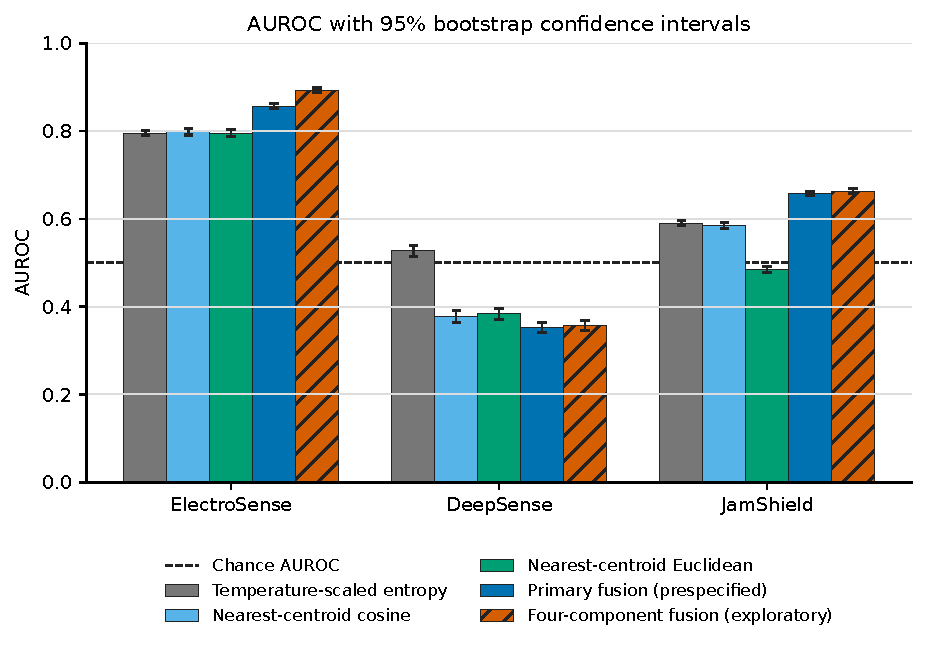
\includegraphics[width=\textwidth]{figure_ood_auroc_with_ci.pdf}
  \caption{OOD AUROC with confidence intervals. Point estimates and percentile 95\% bootstrap confidence intervals under the fixed higher-is-more-OOD orientation; the dashed \(\mathrm{AUROC}=0.5\) line marks chance. The three-component fusion is prespecified; the four-component method is exploratory. The primary result is not replaced by any score-negated analysis.}
  \label{fig:ood-auroc}
\end{figure*}

\begin{figure*}[!t]
  \centering
  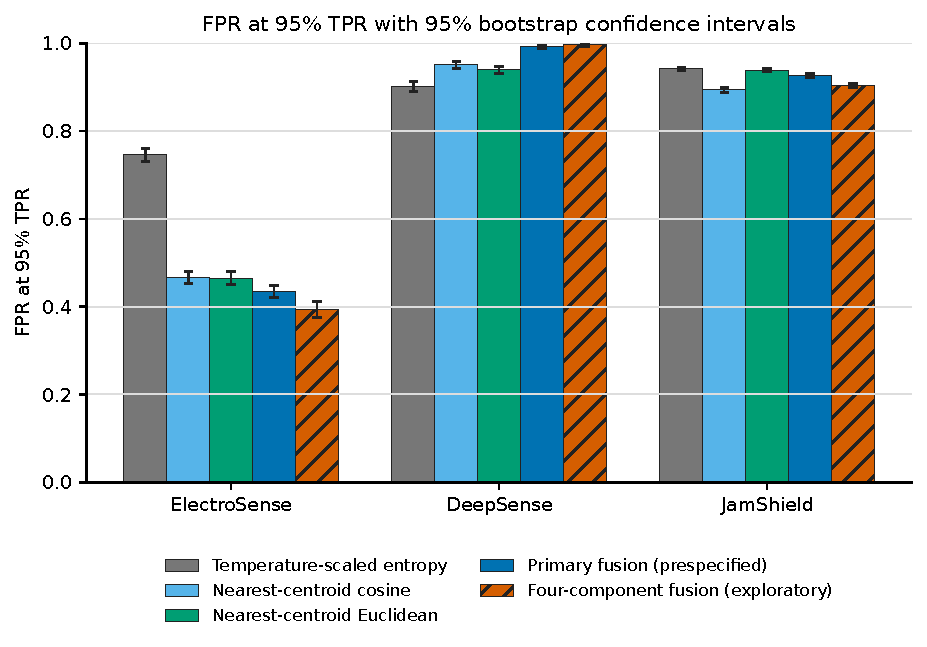
\includegraphics[width=0.91\textwidth]{figure_fpr95_with_ci.pdf}
  \caption{FPR95 with confidence intervals. False-positive rate at 95\% OOD true-positive rate, with percentile 95\% bootstrap confidence intervals under the fixed score orientation. Lower values are preferable; axes include zero and the full probability range.}
  \label{fig:fpr95}
\end{figure*}

\subsection{Paired Comparisons}

Table~\ref{tab:paired-comparisons} states the decision for every reported paired interval. A positive sign means that the left method has a larger metric value; a negative sign means it has a smaller value. For AUROC, AUPR-OOD, and detection accuracy, larger values are ordinarily favorable. For FPR95, smaller values are favorable. Detection-accuracy comparisons remain evaluation-descriptive even when their intervals exclude zero.

\begin{table*}[!t]
  \caption{Paired method differences and interval decisions. Each cell refers to a left-minus-right percentile confidence interval using identical resampling indices within dataset. The comparator set was fixed independently of test performance. A positive sign means that the left method has a larger metric value; a negative sign means it has a smaller value. For AUROC, AUPR-OOD, and detection accuracy, larger values are ordinarily favorable; for FPR95, smaller values are favorable. Exact differences and interval bounds are preserved in the verified paired-differences CSV. Detection-accuracy comparisons are evaluation-descriptive.}
  \label{tab:paired-comparisons}
  \centering
  \scriptsize
  \setlength{\tabcolsep}{2.8pt}
  \renewcommand{\arraystretch}{1.08}
  \newcommand{\ExcludesPositive}{\shortstack{Excludes\\zero (+)}}
  \newcommand{\ExcludesNegative}{\shortstack{Excludes\\zero (\(-\))}}
  \newcommand{\IncludesZero}{\shortstack{Includes\\zero}}
  \begin{tabularx}{\textwidth}{@{}l Y c c c c@{}}
    \toprule
    Dataset & Left-minus-right comparison & AUROC & AUPR-OOD & FPR95 & Detection accuracy \\
    \midrule
    ElectroSense & Primary \(-\) TS entropy & \ExcludesPositive & \ExcludesPositive & \ExcludesNegative & \ExcludesPositive \\
    ElectroSense & Primary \(-\) NC cosine & \ExcludesPositive & \ExcludesPositive & \ExcludesNegative & \ExcludesPositive \\
    ElectroSense & Primary \(-\) NC Euclidean & \ExcludesPositive & \ExcludesPositive & \ExcludesNegative & \ExcludesPositive \\
    ElectroSense & Exploratory four-component \(-\) primary & \ExcludesPositive & \ExcludesPositive & \ExcludesNegative & \ExcludesPositive \\
    \addlinespace
    DeepSense & Primary \(-\) TS entropy & \ExcludesNegative & \ExcludesNegative & \ExcludesPositive & \IncludesZero \\
    DeepSense & Primary \(-\) NC cosine & \ExcludesNegative & \ExcludesNegative & \ExcludesPositive & \IncludesZero \\
    DeepSense & Primary \(-\) NC Euclidean & \ExcludesNegative & \ExcludesNegative & \ExcludesPositive & \ExcludesNegative \\
    DeepSense & Exploratory four-component \(-\) primary & \ExcludesPositive & \ExcludesPositive & \ExcludesPositive & \IncludesZero \\
    \addlinespace
    JamShield & Primary \(-\) TS entropy & \ExcludesPositive & \ExcludesNegative & \ExcludesNegative & \ExcludesPositive \\
    JamShield & Primary \(-\) NC cosine & \ExcludesPositive & \ExcludesPositive & \ExcludesPositive & \IncludesZero \\
    JamShield & Primary \(-\) NC Euclidean & \ExcludesPositive & \ExcludesPositive & \ExcludesNegative & \ExcludesPositive \\
    JamShield & Exploratory four-component \(-\) primary & \ExcludesPositive & \ExcludesNegative & \ExcludesNegative & \ExcludesPositive \\
    \bottomrule
  \end{tabularx}
\end{table*}


For ElectroSense, all primary-versus-comparator intervals exclude zero in the favorable direction: AUROC, AUPR-OOD, and evaluation-descriptive detection accuracy are higher, while FPR95 is lower. The four-component fusion also has favorable intervals relative to the primary method on this dataset, but that result remains exploratory and cannot be used to relabel the primary analysis.

For DeepSense, the primary fusion is worse than every prespecified comparator on AUROC, AUPR-OOD, and FPR95, and all of those intervals exclude zero. Detection-accuracy intervals include zero against temperature-scaled entropy and cosine distance, whereas the interval against Euclidean distance excludes zero in the negative direction. Adding Mahalanobis distance produces exploratory increases in AUROC and AUPR-OOD whose intervals exclude zero, but it also increases FPR95 with an interval excluding zero; the detection-accuracy interval includes zero. These differences do not repair the fixed-orientation failure.

For JamShield, primary-fusion AUROC is higher than each prespecified comparator and each AUROC interval excludes zero. The other metrics expose a trade-off. Against temperature-scaled entropy, primary AUPR-OOD is lower while FPR95 is lower, with both intervals excluding zero. Against nearest-centroid cosine, primary AUPR-OOD is higher but FPR95 is also higher, with both intervals excluding zero; the detection-accuracy interval includes zero. Against Euclidean distance, the primary method is favorable on all reported metrics and every interval excludes zero. The exploratory Mahalanobis addition increases AUROC and evaluation-descriptive detection accuracy and lowers FPR95, but lowers AUPR-OOD; each of those paired intervals excludes zero. Thus JamShield does not support a claim that fusion uniformly improves every metric against every comparator.

\begin{figure*}[!t]
  \centering
  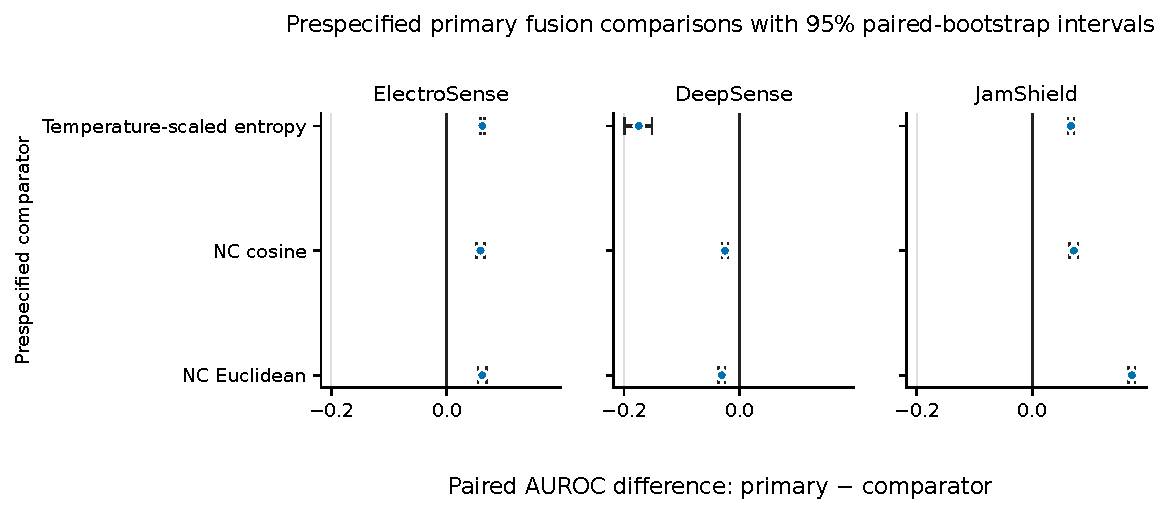
\includegraphics[width=0.98\textwidth]{figure_primary_fusion_comparison.pdf}
  \caption{Primary fusion comparison. This figure reports AUROC only. Paired AUROC differences compare the prespecified primary fusion with each prespecified comparator. Intervals use identical bootstrap resamples across methods; the focused difference scale is centered on zero. The shared horizontal label is \textquotedblleft{}Paired AUROC difference: primary \(-\) comparator.\textquotedblright{}}
  \label{fig:primary-comparison}
\end{figure*}

\subsection{Score Distributions and the DeepSense Inversion}

The dataset-specific score distributions in Fig.~\ref{fig:score-distributions} provide a qualitative view of the fixed orientation. Their score and density axes are independently scaled and must not be compared as common units across datasets. ElectroSense shows useful separation under the primary fusion; JamShield shows partial overlap consistent with its mixed operating metrics; and DeepSense shows a direction mismatch rather than merely broad uncertainty.

DeepSense is retained as a negative fixed-orientation result. Fig.~\ref{fig:deepsense-inversion} compares the original scores with post-hoc negated scores solely to diagnose inversion. The negated scores were not used to choose the primary method, replace any reported value, or make a primary performance claim. The diagnostic suggests that held-out day-two samples can lie closer to training prototypes or receive lower uncertainty than retained day-one test samples under the current representation.

\begin{figure*}[!t]
  \centering
  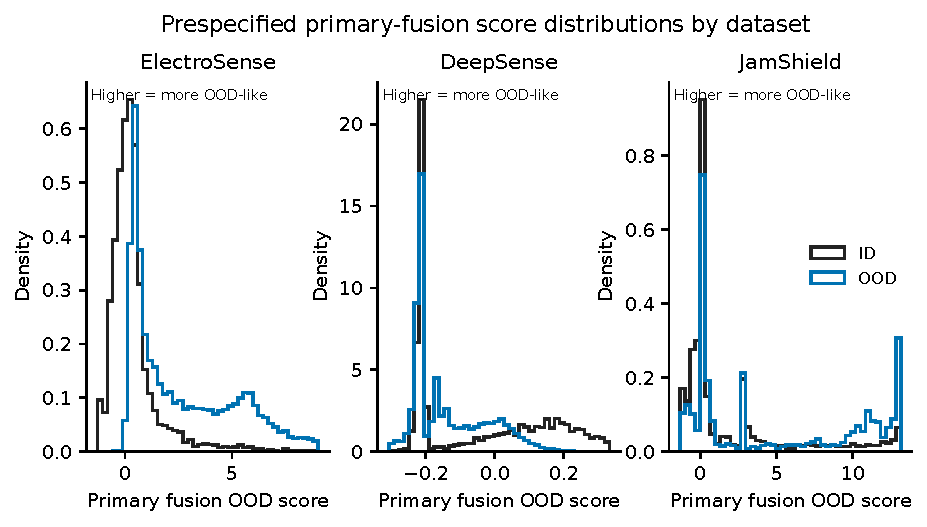
\includegraphics[width=\textwidth]{figure_score_distributions_by_dataset.pdf}
  \caption{Primary-score distributions by dataset. ID and OOD score-density outlines for the prespecified primary fusion, clipped only for display to the 0.5th--99.5th score percentiles within each dataset. Score and density axes are dataset-specific and must not be interpreted as common scales across panels.}
  \label{fig:score-distributions}
\end{figure*}

\begin{figure*}[!t]
  \centering
  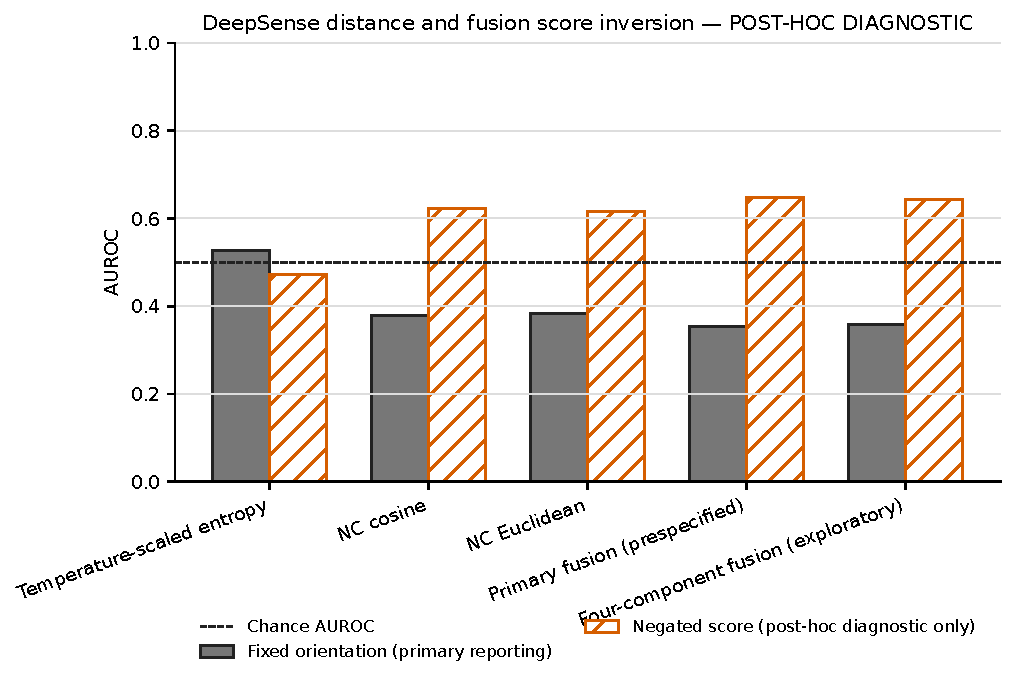
\includegraphics[width=\textwidth]{figure_deepsense_inversion_diagnostic.pdf}
  \caption{DeepSense distance and fusion score inversion---\textbf{POST-HOC DIAGNOSTIC ONLY}. Fixed-orientation AUROC is compared with AUROC after score negation. Negated values are diagnostic only and were not used to change, replace, or reinterpret the primary result.}
  \label{fig:deepsense-inversion}
\end{figure*}

\subsection{Context Across v0--v3}

Table~\ref{tab:stagewise-summary} preserves the stage-wise results used to contextualize the final analysis. The v0 rows cover raw confidence baselines from logistic regression and nearest centroid. The v1 rows cover temperature-scaled logistic-regression entropy and maximum-softmax scores. The v2 rows cover Euclidean, cosine, and Mahalanobis feature distances. The v3 rows contain the prespecified primary fusion and the exploratory four-component ablation. This progression shows that calibration, distance, and fusion alter OOD behavior differently across datasets; it does not define the best method by looking backward at test performance.

\begin{table*}[!t]
  \caption{v0--v3 publication summary. Frozen stage-wise OOD results for raw confidence baselines, temperature-scaled confidence, feature distances, and uncertainty-distance fusion. The three-component v3 method is the prespecified primary analysis; the Mahalanobis four-component method is exploratory.}
  \label{tab:stagewise-summary}
  \centering
  \fontsize{6.4}{7.2}\selectfont
  \setlength{\tabcolsep}{2.4pt}
  \renewcommand{\arraystretch}{0.96}
  \begin{tabularx}{\textwidth}{@{}c c Y r r r r c@{}}
    \toprule
    Stage & Data & Score method & AUROC & AUPR-OOD & FPR95 & Det.\ acc. & Role \\
    \midrule
    v0 & DS & LR entropy & 0.483999 & 0.803427 & 0.922188 & 0.833333 & C \\
    v0 & DS & LR maximum softmax probability & 0.483857 & 0.804785 & 0.922188 & 0.833333 & C \\
    v0 & DS & NC entropy & 0.581740 & 0.840774 & 0.689063 & 0.861354 & C \\
    v0 & DS & NC maximum softmax probability & 0.652601 & 0.897748 & 0.756563 & 0.846667 & C \\
    v0 & ES & LR entropy & 0.795915 & 0.914413 & 0.742808 & 0.771148 & C \\
    v0 & ES & LR maximum softmax probability & 0.795837 & 0.914227 & 0.742808 & 0.771282 & C \\
    v0 & ES & NC entropy & 0.731201 & 0.840276 & 0.643322 & 0.797320 & C \\
    v0 & ES & NC maximum softmax probability & 0.734348 & 0.838485 & 0.601712 & 0.809826 & C \\
    v0 & JS & LR entropy & 0.590865 & 0.716855 & 0.942136 & 0.618468 & C \\
    v0 & JS & LR maximum softmax probability & 0.590865 & 0.716855 & 0.942136 & 0.618468 & C \\
    v0 & JS & NC entropy & 0.556382 & 0.612281 & 0.940553 & 0.689179 & C \\
    v0 & JS & NC maximum softmax probability & 0.556382 & 0.612281 & 0.940553 & 0.689179 & C \\
    \addlinespace
    v1 & DS & Temperature-scaled LR entropy & 0.527378 & 0.822862 & 0.902188 & 0.833333 & C \\
    v1 & DS & Temperature-scaled LR maximum softmax probability & 0.505368 & 0.810584 & 0.920000 & 0.833333 & C \\
    v1 & ES & Temperature-scaled LR entropy & 0.795345 & 0.914816 & 0.745719 & 0.769942 & C \\
    v1 & ES & Temperature-scaled LR maximum softmax probability & 0.795090 & 0.914278 & 0.744007 & 0.770165 & C \\
    v1 & JS & Temperature-scaled LR entropy & 0.590533 & 0.716634 & 0.942136 & 0.618468 & C \\
    v1 & JS & Temperature-scaled LR maximum softmax probability & 0.590533 & 0.716634 & 0.942136 & 0.618468 & C \\
    \addlinespace
    v2 & DS & Mahalanobis & 0.409787 & 0.757572 & 0.939688 & 0.843281 & C \\
    v2 & DS & Nearest-centroid cosine & 0.378069 & 0.745347 & 0.951562 & 0.833333 & C \\
    v2 & DS & Nearest-centroid Euclidean & 0.383826 & 0.746319 & 0.939688 & 0.842396 & C \\
    v2 & ES & Mahalanobis & 0.771683 & 0.902674 & 0.815411 & 0.765699 & C \\
    v2 & ES & Nearest-centroid cosine & 0.798722 & 0.877693 & 0.466267 & 0.844484 & C \\
    v2 & ES & Nearest-centroid Euclidean & 0.795617 & 0.863038 & 0.464384 & 0.842296 & C \\
    v2 & JS & Mahalanobis & 0.475216 & 0.582084 & 0.920325 & 0.587057 & C \\
    v2 & JS & Nearest-centroid cosine & 0.585667 & 0.594142 & 0.894110 & 0.639195 & C \\
    v2 & JS & Nearest-centroid Euclidean & 0.485118 & 0.539054 & 0.939177 & 0.612122 & C \\
    \addlinespace
    v3 & DS & TS entropy + cosine + Euclidean & 0.352958 & 0.737936 & 0.992188 & 0.833490 & P \\
    v3 & DS & Primary + Mahalanobis & 0.357490 & 0.739380 & 0.996250 & 0.833490 & E \\
    v3 & ES & TS entropy + cosine + Euclidean & 0.857037 & 0.934429 & 0.434589 & 0.856632 & P \\
    v3 & ES & Primary + Mahalanobis & 0.893312 & 0.949018 & 0.393322 & 0.862841 & E \\
    v3 & JS & TS entropy + cosine + Euclidean & 0.657625 & 0.710403 & 0.927205 & 0.634887 & P \\
    v3 & JS & Primary + Mahalanobis & 0.663391 & 0.705880 & 0.903674 & 0.642630 & E \\
    \bottomrule
  \end{tabularx}

  \vspace{2pt}
  \parbox{\textwidth}{\fontsize{6.4}{7.2}\selectfont
  DS: DeepSense; ES: ElectroSense; JS: JamShield; LR: logistic regression; NC: nearest centroid; C: contextual comparator; P: prespecified primary (\method{ts_entropy_cosine_euclidean}); E: exploratory ablation (\method{ts_entropy_cosine_euclidean_mahalanobis}). All scores use the fixed higher-is-more-OOD orientation. Detection accuracy (Det.\ acc.) is evaluation-descriptive because its threshold was selected on evaluation data.}
\end{table*}


\section{Discussion}
\label{sec:discussion}

\subsection{Calibration and OOD Separation Are Distinct}

Temperature scaling is valuable because it supplies an explicit, validation-fitted calibration baseline without retraining the classifier~\cite{guo2017calibration}. Its objective, however, is ID validation likelihood. It cannot guarantee that unseen classes or domains receive higher entropy than retained ID samples. The DeepSense and JamShield results make this distinction operational: a confidence transformation can be well specified and leak-free while the target shift remains weakly separated. Claims about calibrated confidence should therefore be accompanied by direct OOD and selective-prediction evaluation~\cite{elyaniv2010foundations,geifman2017selective}.

\subsection{When Uncertainty and Geometry Complement Each Other}

ElectroSense supports the intended complementarity. The class-novelty protocol lets entropy and prototype distances contribute distinct evidence, and the primary fusion improves the reported comparison metrics relative to each standalone prespecified comparator. This is evidence for the frozen ElectroSense protocol, not proof that the same combination will generalize to every modulation, sensor, or frequency regime.

The standalone temperature-scaled entropy, cosine-distance, and Euclidean-distance methods were prespecified comparators because they are the constituent evidence sources of the primary fusion. Their comparison therefore tests complementarity relative to those components; it does not establish superiority over the complete OOD literature. The v0--v2 results provide contextual baselines but were not retrospectively selected as primary competitors. Adding a new external baseline post hoc merely to improve the paper would conflict with the frozen protocol; broader comparisons should instead be prespecified in future work.

JamShield offers a more qualified result. Fusion improves AUROC against all prespecified comparators, suggesting better global ordering of retained and held-out scenarios. Yet AUPR-OOD and FPR95 move differently depending on the comparator. This is not contradictory: AUROC averages ranking behavior across operating points, AUPR-OOD depends on positive-class retrieval and prevalence, and FPR95 emphasizes a high-recall region. A deployment decision should therefore specify the relevant operating metric rather than treating AUROC as a complete substitute.

\subsection{Geometry Can Invert Under Domain Shift}

The DeepSense result is scientifically important because it falsifies the simple assumption that a held-out domain must be farther from training prototypes. Its below-prevalence AUPR-OOD and near-trivial evaluation-descriptive detection accuracy reinforce that fixed-orientation failure rather than providing evidence of a usable operating point. A day shift can move both ID-like and OOD-labeled samples so that the held-out day becomes more concentrated around class centroids than the retained ID test set. Robust validation normalization aligns component scales but cannot correct a direction that reverses after deployment. Reversing the score after seeing OOD labels would produce a useful diagnostic but an invalid primary detector.

A next-step method should be prespecified and validation-identifiable. Candidate directions include two-sided tail scores, validation-fitted density or likelihood-ratio models, and domain-robust representations. Generative-model likelihood inversion and corrective likelihood-ratio scoring illustrate why one-sided scores can fail~\cite{nalisnick2019deep,ren2019likelihood}. Such methods must be selected without target OOD labels and evaluated on untouched shifts.

\subsection{Interpreting the Exploratory Mahalanobis Component}

The exploratory four-component fusion sometimes changes AUROC in a favorable direction, but its effects are not uniform across AUPR-OOD and FPR95. A shared covariance model can emphasize feature directions that help one shift while degrading another operating region. Because this component was not the prespecified primary method, its intervals should motivate a future preregistered comparison rather than retroactively redefine the present claim.

\subsection{Statistical Scope}

Paired intervals exploit exact sample alignment and provide a direct uncertainty estimate for each fixed comparison. Interval exclusion of zero is reported explicitly, but it is not labeled universal statistical significance. The intervals are pointwise, multiple metrics and comparisons are shown, and no family-wise adjustment is applied. The bootstrap also remains conditional on the observed samples; it does not quantify uncertainty over unseen datasets, sensors, or acquisition campaigns.

\section{Limitations}
\label{sec:limitations}

The evaluation uses a single frozen split for each dataset. This supports reproducibility but limits claims about alternative class partitions, days, sensors, or jammer scenarios. The bootstrap captures sampling variation conditional on those evaluation rows and not the broader uncertainty of future domain shifts.

The title's multi-view framing is realized here as heterogeneous dataset representations and fusion of uncertainty and geometric score views. The current experiment does not train a single model that jointly consumes raw I/Q, PSD, spectrogram, and tabular views for each sample. Each dataset contributes its available processed representation, so cross-dataset performance differences may reflect both protocol difficulty and representation quality.

The supervised uncertainty path is based on a lightweight logistic-regression classifier and probability-derived temperature scaling. The verified publication comparison does not include a logit-energy model, deep ensemble, Monte Carlo dropout model, or learned uncertainty head. The feature-distance methods use the existing processed feature space; Euclidean and cosine scores assume useful class prototypes, and Mahalanobis scoring uses a regularized shared covariance model.

Equal fusion weights and the higher-is-more-OOD direction are fixed. This avoids target leakage but does not establish that equal weighting is optimal. The DeepSense result shows that a fixed one-sided distance assumption can fail under domain shift. The score-negation analysis is post-hoc diagnostic only and cannot be considered evidence for a deployable orientation-selection rule.

Detection accuracy is evaluation-descriptive because its threshold is optimized on the same evaluation sample. It should not be used as a claimed deployment operating point. FPR95 is more directly tied to a stated OOD recall target, but it can still be unstable under shifts in prevalence or score distribution.

The stable-order AUPR-OOD implementation retains input order within score ties. It is applied consistently across every method and bootstrap replicate, but it may differ from grouped-threshold implementations when ties are common. Reproduction and external comparison require preserving or explicitly translating this convention.

Finally, the paired intervals are pointwise and unadjusted for the family of datasets, metrics, and comparisons. An interval excluding zero supports only its listed comparison. The current evidence does not justify universal generalization, universal superiority, or a causal explanation for the observed score geometry.

\section{Conclusion}
\label{sec:conclusion}

This study integrates calibrated predictive uncertainty and train-fitted feature distance into a leak-resistant OOD evaluation pipeline for OpenEW-SA RF artifacts. Validation-only temperature scaling and robust normalization make the procedure reproducible without consulting target OOD labels, and equal-weight fusion provides a simple prespecified test of complementary evidence.

The results are deliberately mixed. The primary fusion is effective for ElectroSense class novelty and improves JamShield AUROC against the prespecified comparators, but JamShield retains metric-specific trade-offs. DeepSense remains a negative result under the fixed orientation, and post-hoc negation is diagnostic only. The central conclusion is therefore not that one fused score solves open-set RF monitoring. It is that closed-set calibration, feature geometry, and OOD operating behavior must be measured separately, combined without target leakage, and interpreted at the level of the actual dataset and shift.

\section{Reproducibility Statement}
\label{sec:reproducibility}

All manuscript results are derived from the frozen Paper 2 v0--v3 artifacts and the verified publication-analysis package. The source tables are \path{tables/paper2_v3_bootstrap_confidence_intervals.csv}, \path{tables/paper2_v3_paired_differences.csv}, and \path{tables/paper2_v0_v3_publication_summary.csv}. The independent review report, deterministic bootstrap metadata, validation report, publication figures, and SHA256 manifest are stored in the same package. The local path needed to audit these sources is recorded only in the package README and is intentionally omitted from this submission-facing manuscript.

Repository scripts document manifest construction, split generation, supervised prediction, temperature scaling, entropy extraction, feature-distance scoring, validation-only fusion, metric computation, bootstrap analysis, and publication finalization. The split and score readers preserve \method{sample_id}, labels, domains, and split identifiers as strings; the publication validator explicitly checks DeepSense leading-zero occupancy labels. All compared methods use exact within-dataset sample alignment and the fixed higher-is-more-OOD orientation.

The prespecified method and analysis roles are named in machine-readable metadata. The primary score is \method{ts_entropy_cosine_euclidean}; the Mahalanobis-augmented method is exploratory; and the DeepSense negation is post-hoc diagnostic only. Detection accuracy is marked evaluation-descriptive in the generated tables. The numerical traceability matrix maps every empirical value reported in this manuscript to its source CSV row and columns.

This manuscript integration does not rerun model training, OOD score generation, or bootstrap sampling. It reads the verified tables and leaves Paper 1 and all frozen Paper 2 snapshots unchanged. Repository-level validation and remaining editorial tasks are recorded in \path{manuscript_completion_checklist.md}.


\section*{Declarations}
\noindent\textbf{Conflict of Interest:} \submissionplaceholder{conflict-of-interest statement}.

\noindent\textbf{Data Availability:} \submissionplaceholder{data-availability and data-license statement}.

\noindent\textbf{Code Availability:} \submissionplaceholder{code-availability, repository/version, and license statement}.

\section*{Acknowledgments}
\submissionplaceholder{acknowledgments}.

\begin{thebibliography}{17}
\bibitem{R1}\textbf{[REFERENCE NEEDED: R1]} Authoritative RF spectrum-monitoring review, standards document, or primary field study.
\bibitem{R2}\textbf{[REFERENCE NEEDED: R2]} Foundational or peer-reviewed OOD/calibration study.
\bibitem{R3}\textbf{[REFERENCE NEEDED: R3]} Peer-reviewed OOD/open-set evaluation-protocol or model-selection guidance.
\bibitem{R4}\textbf{[REFERENCE NEEDED: R4]} Foundational open-set recognition paper or authoritative survey.
\bibitem{R5}\textbf{[REFERENCE NEEDED: R5]} RF OOD/domain-generalization survey or primary RF studies.
\bibitem{R6}\textbf{[REFERENCE NEEDED: R6]} Original confidence/OOD baseline papers or an authoritative benchmark.
\bibitem{R7}\textbf{[REFERENCE NEEDED: R7]} Original temperature-scaling/calibration paper and, if needed, an OOD-calibration study.
\bibitem{R8}\textbf{[REFERENCE NEEDED: R8]} Original energy-based OOD detection paper.
\bibitem{R9}\textbf{[REFERENCE NEEDED: R9]} Foundational prototype/open-set or feature-distance OOD work.
\bibitem{R10}\textbf{[REFERENCE NEEDED: R10]} Canonical Mahalanobis OOD paper and, if required, a numerical-method source.
\bibitem{R11}\textbf{[REFERENCE NEEDED: R11]} Authoritative OOD benchmark or metric-methodology reference.
\bibitem{R12}\textbf{[REFERENCE NEEDED: R12]} Statistical bootstrap reference and paired-model-comparison guidance.
\bibitem{R13}\textbf{[REFERENCE NEEDED: R13]} Primary ElectroSense dataset publication and official dataset record.
\bibitem{R14}\textbf{[REFERENCE NEEDED: R14]} Primary DeepSense dataset publication and official dataset record.
\bibitem{R15}\textbf{[REFERENCE NEEDED: R15]} Primary JamShield dataset publication and official dataset record.
\bibitem{R16}\textbf{[REFERENCE NEEDED: R16]} Foundational selective-classification or risk-coverage reference.
\bibitem{R17}\textbf{[REFERENCE NEEDED: R17]} Peer-reviewed typicality, density-based OOD, or two-sided anomaly-detection work.
\end{thebibliography}

\end{document}
